%!TEX root = ../../main.tex

\chapter{Photoluminescence Setup}	\label{ch::pl_setup}
\chaptermark{Experimental Setup}

	\begin{remark}
		\item Fill in missing values described as todos.
	\end{remark}


	The study and handling of \sivs in \nds requires dedicated experimental methods and techniques. In the following we detail the experimental setup used to obtain the results presented in later chapters. The core of the setup consists of a confocal microscope connected to either a grating spectrometer or a \HBT interferometer. The former yields fluorescent spectra of \sivs while the latter enables measurements of the intensity autocorrelation function of individual emitted fluorescent photons.

	\section{Confocal Setup} \label{sec::confocal}

		When studying \sivs experimentally, two capabilities are key: Exciting \sivs into emitting fluorescent light using a laser and the ability to register resulting \siv fluorescence. A confocal setup elegantly supports both requirements. Confocal microscopy uses an objective to focus a laser onto a small volume of a sample which can be used to excite \sivs in a controlled fashion. As the luminescence light returning from the emitter is in the same focus as the excitation laser light, it is effectively collected by the objective, thus the designation ``confocal". For an overview of confocal microscopy we refer the reader to \cite{webb1996confocal}.

		\begin{figure}[htb]
			\centering
			\testbox{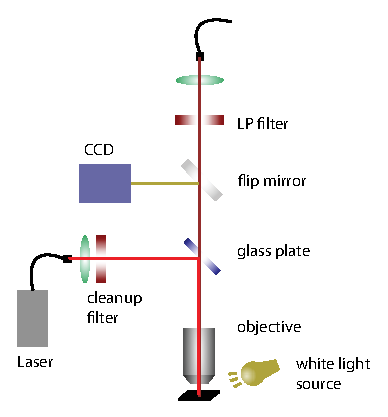
\includegraphics[trim = 0 0 0 0,  clip= true, width = 0.5\textwidth]{./pics/confocal_setup_small.eps}}
			\caption[Confocal microscopy setup]{Confocal microscopy setup. An excitation laser beam (red) leaves an optical fiber and is directed towards a glass plate. The glass plate reflects $\approx \SI{10}{\percent}$ of the incoming beam towards an objective after which is focused onto the sample. The same objective collects the resulting fluorescent light and redirects it towards the glass plate where $\approx \SI{90}{\percent}$ of the light is allowed to pass. The passing \fl light is fed into an optical fiber which connects to the detection part of the setup. A flip mirror can be engaged to bring a CCD camera into the setup in case a white light source is used to illuminate the sample.}
			\label{fig::confocal_setup}
		\end{figure}

		\autoref{fig::confocal_setup} illustrates the confocal setup deployed in this work.
		With the exception of the laser and the sample stage, the whole setup is fixed to a vertical breadboard.
		The vertical design permits a horizontal sample stage, promoting quick scanning and exchanging of samples.
		The sample itself resides on top of a translation stage and is held in place sufficiently by surface friction.
		It is oriented by an aluminum angle adjustable via a manual rotation stage.
		The translation stage is moved by two stepper motors (Newport MVP25XL) enabling the sample to be translated horizontally, i.e.\ in the $x-y$ plane.
		Above the horizontal stage, the objective is fixed to another stage which in turn is mounted to a vertical breadboard.
		In this way, the vertical distance between the sample and the objective can be controlled. As a result the focus of the laser can be adjusted along the $z$ axis, \i.e.\ the optical axis, allowing to implement a full three-axis scan of samples.
		\\
		The bright red color in the sketch in \autoref{fig::confocal_setup} represents the path of the excitation laser beam.
		The sample is excited with a continuous wave diode laser (Sch\"after-Kirchhoff, 58FCM) emitting at a \wl of \SI{660}{\nano\meter}.
		The outlet of the laser is a pigtail fiber.
		The laser light is out-coupled and collimated by an aspheric lens.
		To suppress sideband emission from the laser, a \SI{660}{\nm} bandpass filter with a filter window of \SI{10}{\nm} is used.
		After this cleanup filter, the excitation beam hits a \SI{}{\milli\meter} glass plate (fabricator Halle Germany \todo[fancyline]{thickness}) redirecting the beam. It is then focused onto the sample by a $100 \times$ microscope objective (Olympus, LMPlanFLN) with a numerical aperture of $0.8$.
		\\
		The collected light follows the detection beam path depicted in dark red in \autoref{fig::confocal_setup}.
		Both the excitation light reflected from the sample surface and the \fl from the color centers pass through the glass plate.
		Removing the flip mirror behind the beamsplitter from the path directs light towards a \smf (Thorlabs SM600) connecting the confocal setup with either the spectrometer or the \hbt setup. Prior to focusing light into the \smf using an aspheric lens, a long-pass filter is deployed to eliminate residual excitation light and ambient light.
		The filter is chosen with a cutoff \wl of \SI{710}{\nm} or \SI{720}{\nm}.
		Besides the obvious purpose of guiding the \pl light to the spectrometer and the \HBT setup for spectroscopic investigations, it severs another crucial purpose. Namely, diameter of about \SI{4.3}{\micro\meter} acts as a pinhole to reject \pl light from depths outside of the focal plane \cite{Santori2010}.
		For this axis the resolution amounts to \todo[fancyline]{resolution value}, in the plane of the sample it is \todo[fancyline]{resolution value}.

		We remark that the glass plate in used \autoref{fig::confocal_setup} has a high transmission of $\approx \SI{90}{\percent}$. This leads to a high collection efficiency of \fl light at the cost of excitation efficiency since most of the exciting light is not being redirected towards the sample. In contrast to that, certain use cases such as saturation measurements require high excitation intensities. To realize these the glass plate may be replaced by a dichroic mirror (DRLP692). A dichroic mirror spectrally separates excitation light from \pl light as it selectively transmits and reflects light as a function of its wavelength.

		In general, if high excitation setting is required we opt for a dichroic mirror, otherwise working with the glass plate at lower excitation is the default. This is advised since high intensities carry the danger of damaging \sivs to the point of bleaching and can also cause fluorescent intermittence of \sivs, \i.e.\ blinking, as an unwanted side-effect see \autoref{ch::siv}.

	\section[Surface Imaging]{Optical Imaging of The Sample Surface} \label{sec::methods_optical}

		The setup introduced in the previous section can be modified to investigate the sample surface before starting fluorescence measurements.
		For this purpose, the sample is directly illuminated at a flat angle from outside the objective with white light from a halogen lamp, see the white light source in \autoref{fig::confocal_setup}.
		The flip mirror behind the glass plate is brought into an upright position to guide the light towards a CCD camera.
		The scattered light from the sample surface is collected by the objective and the surface is imaged on the CCD chip.
		Thus \nds and other features on the substrate are made visible.
		The resolution of this configuration of the setup is limited by \todo[fancyline]{optical diffraction, shadows}.

		\begin{figure}[htb]
			\centering
			\testbox{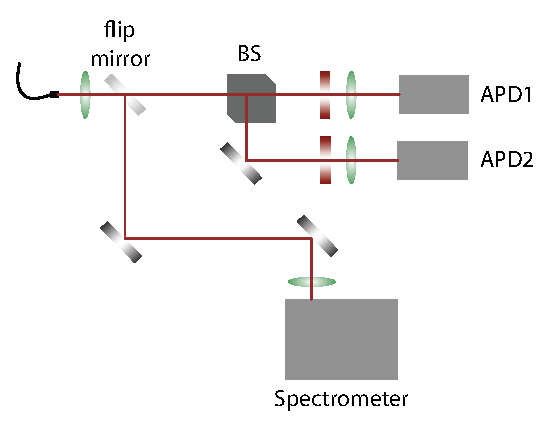
\includegraphics[trim = 0 0 0 0,  clip= true, width = 0.5\textwidth]{./pics/hbt_spectrometer.eps}}
			\caption[Spectrometer and HBT setup]{Spectrometer and HBT interferometer. Fluorescent light arrives via an optical fiber and is directed towards a flip mirror. The mirror directs the beam either towards a 50:50 beam splitter (BS) into the APDs of the HBT setup, or into a grating spectrometer.}
			\label{fig::hbt_spectrometer}
		\end{figure}

		In chapter \autoref{ch::coupling} we introduce applications of \sivs in \nds, for which knowing the precise positions of specific \nds is crucial.
		Therefore, cross markers are milled into the surface of the substrate on which the \nds are situated.
		These markers of a size of \SI{10}{\micro\meter} can easily be recognized by optical imaging and can thus be used as landmarks for the purpose of indexing individual \sivs.
		The starting point for a scan of an area of interest on the sample is fixed while navigating with the optical image.
		After flipping the flip mirror, light is directed towards the detection part of the setup enabling systematic scans of the sample.

	\section{Spectrometer} \label{sec::methods_spectrometer}

		\autoref{fig::hbt_spectrometer} displays the detection part of the setup.
		The \fl arrives via a pigtail fiber connecting the confocal setup with the detection setup and is out-coupled with an aspheric lens.
		A flip mirror is employed to direct the light either to a grating spectrometer or the \hbt setup.
		The optical spectrum of a light source gives insight to the optically active constituents and therefore bears information about the emitter.

		As mentioned before, the \fl from the \sivs is investigated with the grating spectrometer (Princeton Instruments Acton2500i).
		The incident beam passes through an entrance slit, is then scattered on the grating where the light is spectrally divided and finally hits a detector, imaging the entrance slit on the detector surface.
		The employed detector is a CCD camera (Princeton Instruments, Spec-10) cooled with liquid nitrogen to a temperature of \SI{-120}{\celsius}. This limits background signals due to thermally generated free charge carriers.
		The spectrometer is optimized for detection of light up to a \wl of \SI{900}{nm}.
		and features three gratings: \SI[per-mode=symbol]{600}{\lines\per\mm}, \SI[per-mode=symbol]{1200}{\lines\per\mm}, and \SI[per-mode=symbol]{1800}{\lines\per\mm}.
		These gratings are mounted on a turret, allowing easy swapping of gratings between measurements.

		With the spectrometer's step-and-glue function which is implemented in the spectrometer software (WinSpec) it is possible, to record several spectra over a wide \wl range which are then stitched together.
		It is therefore possible to combine a larger \wl range with a higher resolution.
		For most measurements the grating with \SI[per-mode=symbol]{600}{\lines\per\mm} was used.
		The resolution of the spectrometer using the \SI{600}{\lines\per\mm} is \SI{0.13}{nm} at \SI{738}{nm} and the accuracy amounts to \num{\pm0.4} as stated by the manufacturer.
		This resolution suffices for the measurements presented in this work.

	\section[HBT]{\HBT Setup}\label{sec::methods_hbt}

		A \HBT setup is used to establish the intensity autocorrelation function (\gt function) of an emitter \cite{brown1956correlation, brown1956test}.
		In this work, the \gtf is used to assert the non-classical behavior of a \pl source, \i.e.\ characterize its behavior as a single photon emitter.
		In the photon number representation, it is defined as follows:

		\begin{equation}
		\gt(\tau) = \frac{ \mean{ N(t) N(t+\tau) } }{\mean{N(t)}^2}.
		\end{equation}

		Here, $N(t)$ denotes the number of photons at a certain time $t$, $N(t+\tau)$ denotes the number of photon at a time interval $\tau$ later than $t$.
		The angular brackets $\mean{}$ denote temporal averaging.
		For a two-level system $\gt(\tau)$ can be interpreted as the probability of detecting two photons separated by a time interval $\tau$.
		The physical intuition behind this definition is as follows: The detection of a fluorescent photon emitted from a quantum system is the result of an excited electron relaxing back to its ground state. To emit a consecutive single photon, an additional electron must first be promoted to an exited state, a process which takes a certain amount of time, see \autoref{ch::theory}. If $\gt(\tau) \neq 0$ in the limit of $\tau \to 0$ a system is capable of emitting several photons simultaneously. This is known as photon bunching and is typical for classical light sources. In contrast, $\gt(\tau) \to 0$ for $\tau \to 0$ is an indication that no two photons can be detected simultaneously. This property is termed photon anti-bunching and is a defining characteristic of non-classical light sources such as \sps. The last important type are coherent photons, as for instance produced via stimulated emission. \autoref{fig::g2_illustration} shows how the \gt function distinguishes these three types. For an in-dept review of the intensity auto-correlation function we refer the reader to \cite{Neu2012, Fox2006}.

		\begin{figure}[htb]
			\centering
			\testbox{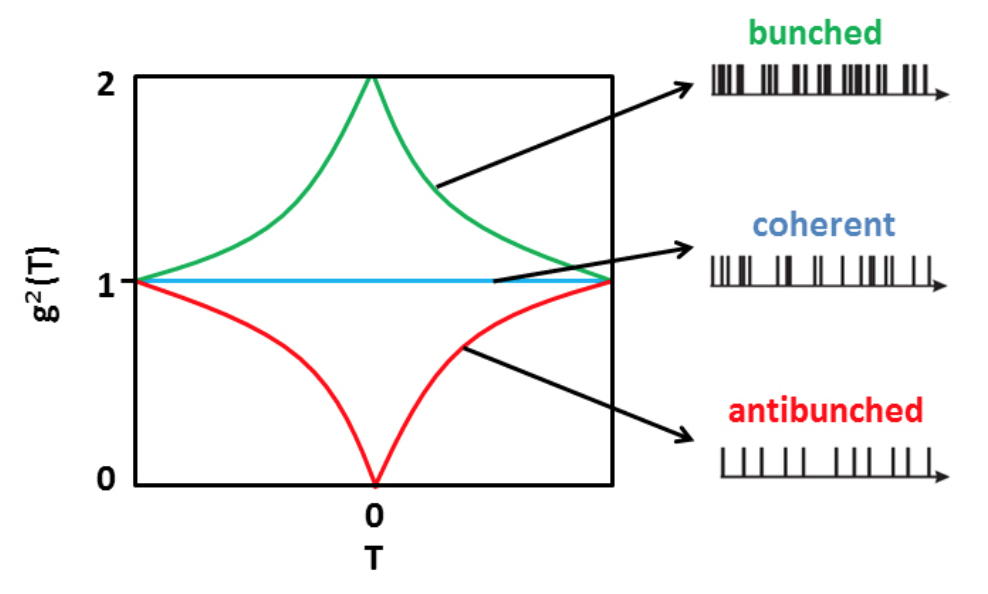
\includegraphics[trim = 0 0 0 0,  clip= true, width = 0.5\textwidth]{./pics/g2_function_illustration.png}}
			\caption[Sketch of typical \gt functions]{Intensity autocorrelation function for coherent, bunched, and anti-bunched light sources. Figure and caption reproduced from \cite{rahbany2016towards}.}
			\label{fig::g2_illustration}
		\end{figure}


		The aim of the \hbt setup is to record the time delay between two consecutive photons as a prerequisite to compute $\gtz$.
		A sketch of the \hbt setup is shown in \autoref{fig::hbt_spectrometer}.
		Photons are detected using single photon \apds (\APDs, PicoQuant $\tau${}-SPAD100).
		\APDs are the semiconductor analog to photomultiplier tubes, i.e.\ an incoming photon creates secondary charge carriers through ionization.
		The secondary charge carrier is accelerated by a bias voltage to create further secondary charge carriers, resulting in an avalanche effect.
		Therefore, the signal of a single photon is intensified and detected as an electrical current pulse.
		These \apds have a nominal detection efficiency of up to \SI{70}{\percent} at an optimal wavelength of about \SI{670}{\nm} and a dark count rate of under \SI{100}{\cps}.
		If a charge carrier created by the avalanche is temporarily trapped and later liberated, it induces a so-called after-pulse.
		To avoid detecting these artifacts as real events, the \APDs have a dead time of about \SI{70}{\ns}.
		In the ideal case, one \APD would be enough to measure the time delay between two consecutive photons.
		However, the second of two consecutive photons could hit the detector during its dead time.
		To circumvent this problem, two \APDs are employed and the detection beam is split with a non-polarizing 50:50 beamsplitter cube.
		Each beam then goes through a band-pass filter and is focused on the \apd with an aspheric lens.
		As the beam path is slightly different for each \APD, a small optical path difference is introduced, however, this difference only results in an offset of the \gtf and does not alter the physical nature of the result.
		The bandpass filters serve two purposes:
		First, they limit optical crosstalk between the \apds.
		The detection process in an \apd produces light due to recombination of charge carriers.
		Crosstalk between two \apds occurs, if one of the photons produced by recombination in one \apd escapes and is detected in the other one \cite{Younger2009}.
		Second, the band-pass filters serve to reduce \bkg during the \gt measurement process or to spectrally separate emission from several emitters.
		Therefore, it is possible to find single emitters, which are not spatially separated enough to be separated by the spatial resolution of the setup.
		In particular, emitters can be individually investigated if their \ZPLs exhibit wavelengths which are spectrally well separated.
		Band-pass filters suited for the respective wavelengths are used to selectively investigate light associated with distinct \ZPLs.
		\\
		When the \APD fires, it outputs a digital TTL (transistor-transistor logic compatible) signal.
		The arrival times of the signals, so-called time-tags, are recorded with a time-tag unit (produced by dotfast-consulting) with a temporal resolution of \SI{78.125}{\pico\second}.
		The timing uncertainty of the photon detection process introduces variations of the digital signal's time-tag from the actual detection time.
		This is called timing jitter and adversely affects the recorded time-tags and consequently the value of $\gtz$. In the past it has been shown to significantly obfuscate the detection of anti-bunching behavior in \sps and thus relevant corrections need to be taken into account \cite{Neu2012, Riedrich-moller2014}.
		\\
		As stated earlier, the time delay between two consecutive photons is necessary for the reconstruction of the \gtf.
		The time delays are fed into a histogram which is then fitted to receive the continuous \gtf.
		As a suitable fit function a numerical convolution between the $\gt(\tau)$ derived for a three-level system and detector timing jitter can be used \cite{neu2011single, Neu2012, Riedrich-moller2014}.
		\\
		In the \HBT{}-setup the arrival time of photons are recorded with two APDs, each of which keeping a list of arrival times as raw data.
		To get a single array of arrival times of the photons, which can then be binned to obtain the \gtf, the arrays of time-tags of the two \APDs have to be correlated.
		For that, the time difference between each entry in one array and all consecutive time-tags in the other array are determined and binned according to the timing resolution of the time-tag unit.
		After normalizing and fitting these data, \gtz can be obtained determining whether a emitter characterizes as a \sps.
